\documentclass[paper.tex]{subfiles}

\usepackage{tikz}
\usepackage{amsmath}
\usepackage{graphicx}
\usepackage{tabularx}
\usepackage{multicol}
\usepackage{algpseudocode}
\usepackage{algorithm}

% Add vertical spacing to tables
\renewcommand{\arraystretch}{1.4}

% Begin Document
\begin{document}

\section{Background}

The Minimum Dominating Set of a Graph is defined as the set of vertices for which each vertex or one of its neighbors is in the set.
The size of the minimum set will be unique, however there may be multiple sets of that size that are a minimal covering.
Consider the graph below.

\begin{center}
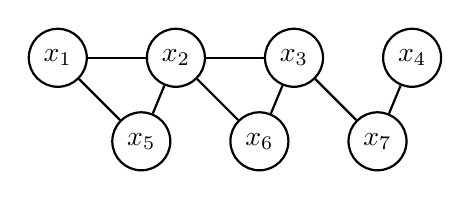
\begin{tikzpicture}[node distance={15mm}, thick, main/.style = {draw, circle}] 
    \node[main] (1) {$x_1$};  
    \node[main] (2) [right of = 1] {$x_2$};  
    \node[main] (3) [right of = 2] {$x_3$};  
    \node[main] (4) [right of = 3] {$x_4$};
    \node[main] (5) [below right of = 1] {$x_5$};
    \node[main] (6) [below right of = 2] {$x_6$};
    \node[main] (7) [below right of = 3] {$x_7$};  
    \draw (1) -- (5);
    \draw (1) -- (2);
    \draw (2) -- (3);
    \draw (2) -- (5);
    \draw (2) -- (6);
    \draw (3) -- (6);
    \draw (3) -- (7);
    \draw (4) -- (7);
\end{tikzpicture}
\end{center}

This graph has minimum dominating sets, $\{x_2,x_4\}$ and $\{x_2,x_7\}$.
The vertex $x_2$ covers vertices $\{x_1,x_3,x_5,x_6\}$, leaving nodes $x_4$ and $x_7$.
Either vertex can dominate the other and complete a covering of the graph.
In this example, both the approximate algorithm and brute force approach would find an equally sized set.

The next section explores the two algorithmic approaches used in this project.


\end{document}